\subsection{Organizzazione del codice}
La suddivisione del codice rispecchia fortemente il design architetturale generale descritto in precedenza.
\begin{center}
    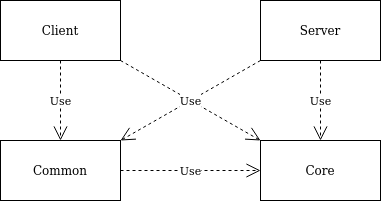
\includegraphics[scale=0.5]{moduli.png}
\end{center}
Sono stati realizzati 4 moduli:
\begin{itemize}
    \item Core: comprende tutte le entità necessarie alla realizzazione del gioco e le regole per poter portare avanti una partita, è l’unico tra i moduli totalmente indipendente dagli altri.
    \item Common: codice comune alle parti di client e server, per la maggior parte definisce i messaggi utilizzati per lo scambio di informazioni
    \item Client: contenente tutto ciò che concerne il client, interfaccia utente, parte di comunicazione con il server e di aggiornamento dello stato della partita
    \item Server: contenente tutta la parte di gestione delle lobby e delle partite in corso
\end{itemize}

\subsection{Core}
Il core modella al suo interno tutte le entità del gioco Machiavelli reale, come le carte, il mazzo e il tavolo da gioco, come anche la GameInterface, cioè un insieme di funzioni che gli altri moduli del progetto devono usare per poter interagire con le entità.
Tali funzioni infatti modellano tutte le azioni che un giocatore può svolgere nel gioco reale.
\textparagraph E’ importante sottolineare il fatto che sia immutabile e quindi non conserva alcuno stato interno.
Esso deve essere utilizzato all’esterno sfruttando appunto le API messe a disposizione.

\subsubsection{Entità}
\begin{center}
    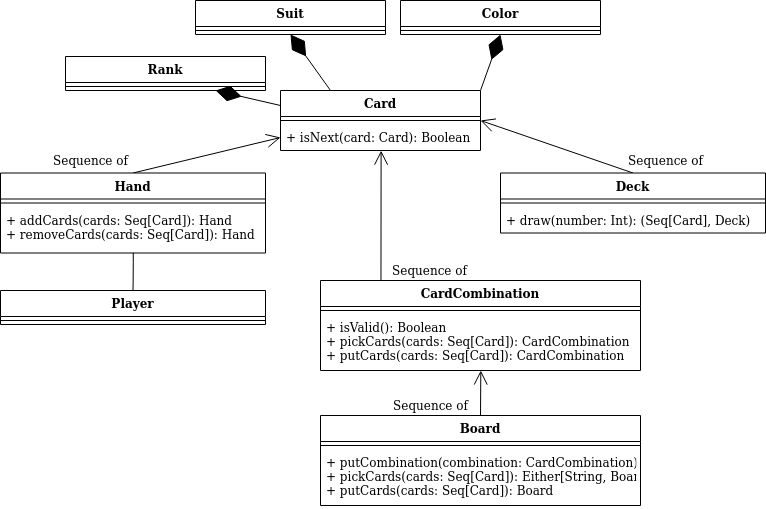
\includegraphics[width=\textwidth]{classi-Page-1.png}
\end{center}
Le entità di gioco sono elencabili come:
\begin{itemize}
    \item Card, corredata da un Rank (valore nominale), un Seme e un Colore.
    E’ stato modellato anche il caso del Rank Asso come 14-esimo possibile valore, per poterne effettuare la validazione qualora si trovasse dopo il Re (13-esimo valore) in una combinazione
    \item Player, composta da un username, un id e una mano
    \item Hand, che contiene i metodi per poter aggiungere (o rimuovere) carte dal tavolo alla mano (dalla mano al tavolo) e per ordinare le carte
    \item CardCombination, rappresenta un tris, poker o una scala ordinata
    \item Deck, rappresenta il mazzo
    \item Board, rappresenta il tavolo di gioco e contiene un insieme di CardCombiantion e i relativi metodi per poterle aggiungere, rimuovere e aggiornare
\end{itemize}

\subsubsection{Prolog}
Per la gestione delle regole di validazione, sii è deciso di utilizzare questo linguaggio in quanto è possibile esprimerle in maniera totalmente dichiarativa conciso ed efficente.
La libreria utilizzata è TuProlog.
\begin{center}
    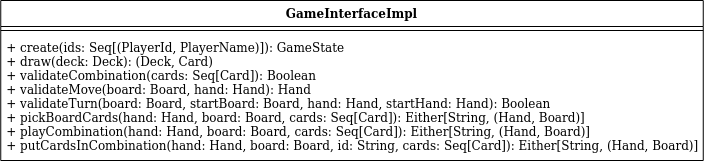
\includegraphics[scale=0.5]{classi-Page-2.png} %TODO: Aggiungere grafico.
\end{center}
Di seguito vengono descritte le classi:
\begin{itemize}
    \item il PrologGame espone tutte le funzionalità implementate attraverso tale linguaggio.
    Ogni qualvolta che si deve eseguire una funzionalità in Prolog, è necessario richiamare un metodo di questa classe corrispondente all’azione di Prolog.
    In particolare permette di creare le carte corredate da un valore, un seme e un colore per formare il deck di gioco, di eseguire la validazione di una sequenza di carte, che sia essa una scala, tris o poker e ne esegue l’ordinamento per seme e per valore.

    \item il PrologEngine esegue effettivamente le azioni di Prolog.
    Si è deciso di realizzare un piccolo DSL che permettesse di facilitare l’utilizzo della libreria TuProlog e di aumentarne l’espressività del codice.
    Dopo aver caricato la specifica teoria, il PrologEngine esegue le funzioni in grado di:
    \begin{itemize}
        \item risolvere un singolo obiettivo o più obiettivi
        \item verificare se un obiettivo ha successo
        \item se vi sono altre soluzioni dopo averne trovata almeno una
        \item estrarre i valori dalle variabili, dopo l’esecuzione di un predicato, tramite il metodo bindingVars
    \end{itemize}

    \item il PrologGameConverter espone le funzioni in grado di formulare obiettivi nel giusto ‘formato’ in Prolog e di convertire il risultato ottenuto dal PrologEngine nel tipo corretto, a seconda dell’utilizzo.
    In particolare, grazie all’utilizzo dell’oggetto PrologUtils, espone metodi in grado di ‘pulire’ (da caratteri non conformi) il risultato del Prolog dopo averlo convertito in stringa.
    Questo è stato reso necessario poiché quando si dava in input un obiettivo che conteneva una lista di tuple (ogni carta è una tupla che contiene nel seguente ordine valore, seme e colore), il risultato risultava essere ‘sporco’ da caratteri estranei rispetto al predicato dato in input.
    Di fatto l’oggetto PrologUtils espone delle funzioni e una Regex che lavorano su stringhe e sostituiscono i caratteri non accettati.
    La classe converter permette infine di gestire la validazione di specifici casi, ad esempio una combinazione contenente uno o più assi.
    Questo perché l’asso in una combinazione che forma una scala, può essere posto prima del due o dopo del re e quindi a fini di validazione, per la teoria definita, l’asso può assumere sia il valore 1, sia il 14.
    Il metodo OptionalValueAce gestisce i casi appena descritti cambiandone il valore in modo conforme.

\end{itemize}

\subsubsection{Game Interface}
\begin{center}
    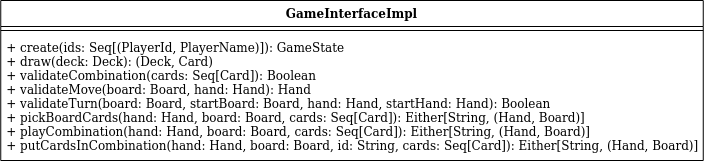
\includegraphics[scale=0.5]{classi-Page-2.png}
\end{center}

\subsection{Client}

\subsubsection{MVC}

\subsubsection{Lobby}

\subsubsection{Game}

\subsection{Server}

\subsubsection{Lobby}

\subsubsection{Game}

\newpage